\documentclass[a4paper,6pt]{article}

\usepackage{amsmath,amsfonts,amssymb,amsthm,epsfig,epstopdf,titling,url,array}
% NEWCOMMAND LIST
\newcommand{\vv}[1]{\ensuremath{\mathbf{#1}}}
\newcommand{\vs}[1]{\ensuremath{\boldsymbol{#1}}}
\newcommand{\sv}[1]{\ensuremath{\boldsymbol{\hat{#1}}}}
\newcommand{\sm}[1]{\ensuremath{\small{#1}}}
\newcommand{\norm}[1]{\ensuremath{\lvert\lvert {#1} \lvert\lvert}}
\newcommand{\Ss}[1]{\ensuremath{[{ #1} \times]}}
\newcommand {\lieB}[2]{\ensuremath{ \big{[}\mathbf{#1},\mathbf{#2} \big{]} } }
\newcommand {\lieD}[2]{\ensuremath{ L_{\mathbf{#1}} #2 } }
\newcommand {\lieDr}[3]{\ensuremath{ L^{#2}_{\mathbf{#1}} #3 } }
\newcommand{\parallelsum}{\mathbin{\!/\mkern-5mu/\!}}


% DEFINITIONS LIST
\theoremstyle{Definition}
\newcounter{Def} \numberwithin{Def}{section}

\newtheorem{stlc} [Def] {Definition} 
\newtheorem{accessibility}[Def]{Definition}
\newtheorem{set_of_reachable_states} [Def]{Definition}
\newtheorem{proper_control_set} [Def]{Definition}
\newtheorem{Lie_derivative}[Def]{Definition}
\newtheorem{Lie_bracket}[Def]{Definition}
\newtheorem{Lie_distribution}[Def]{Definition}
\newtheorem{Bad_Lie_bracket}[Def]{Definition}
\newtheorem{LARC_condition}[Def]{Definition}
\newtheorem{relative_degree}[Def]{Definition}

%THEOREMS LIST
\theoremstyle{Theorem}
\newcounter{Theo} \numberwithin{Theo}{section}

\newtheorem{Sussman_bracketing} [Theo] {Theorem}
\newtheorem{Sussman_controllability} [Theo] {Theorem}
\newtheorem{Input_state}[Theo]{Theorem}
\newtheorem{Lyapunov_lemma2}[Theo]{Theorem}


\pagestyle{empty}

\usepackage{amsmath}
\usepackage{siunitx}
\usepackage{pdflscape}
\usepackage[top=10mm, bottom=10mm, left=5mm, right=5mm]{geometry}
\renewcommand{\theequation}{\thesection.\arabic{equation}}
\usepackage{amsthm}
\usepackage{amsfonts}
\usepackage{framed}
\usepackage{textcomp}
\usepackage{color}
\usepackage[dvipsnames]{xcolor}
\usepackage{mathrsfs}
\usepackage{multirow}
\usepackage{mathabx}
\usepackage{tabulary}
\usepackage{array}
\usepackage{hyperref}
\usepackage{float}
\usepackage{pdflscape}
\usepackage[T1]{fontenc}
\usepackage[british,UKenglish,USenglish,english,american]{babel}
\usepackage[utf8]{inputenc}
\usepackage{graphicx}
\graphicspath{ {images/} }
\usepackage{epstopdf}
\usepackage{longtable}
\usepackage{graphicx}
\usepackage{caption}
\usepackage{subcaption}
\linespread{1}
\usepackage{amssymb}
\usepackage{booktabs}
\usepackage{caption}
\usepackage{tabularx}
\usepackage{adjustbox}
\usepackage{subcaption}

\newcommand{\HRule}{\rule{\linewidth}{0.5mm}}

\begin{document}

\begin{titlepage}
   \vspace*{\stretch{1.0}}
   \begin{center}
      \Large\textbf{ RL \& GA optimizaztion obstacle avoidance recap. }\\
      \large\textit{Matteo Baiguera}
   \end{center}
   \vspace*{\stretch{2.0}}
\end{titlepage}


\begin{abstract}
Aim of this document is to summarize results concerning reinforment learning in the simple obstcle avoidance problematics. Main ingredients:
\begin{enumerate}
\item{\textbf{Obstacle: } a circle of radius $50m$}
\item{\textbf{Robo-sat:} autonomus 2d free-flyer, force to move inside a control-box of dimension $L$  starting from $r_0$ to a goal position $r_{goal}$ avoding the obstacle  }
\item{\textbf{neural-network:} 
\begin{enumerate}
	\item{ normalized inputs: current velocity: $v/ V$, current postion: $r/L$. Where $V$ has been taken reasonably high to ensure $[-1,1]$ \\ !! Possible source of bad performance in training !! }
	\item{ constituted by a single hidden layer. Activation function: $\mathbf{tanh}$ (all possible values)}
\end{enumerate}

 }

\end{enumerate}
\end{abstract}

\section{Baseline: }
\begin{figure}[H]
 	\begin{center}
 		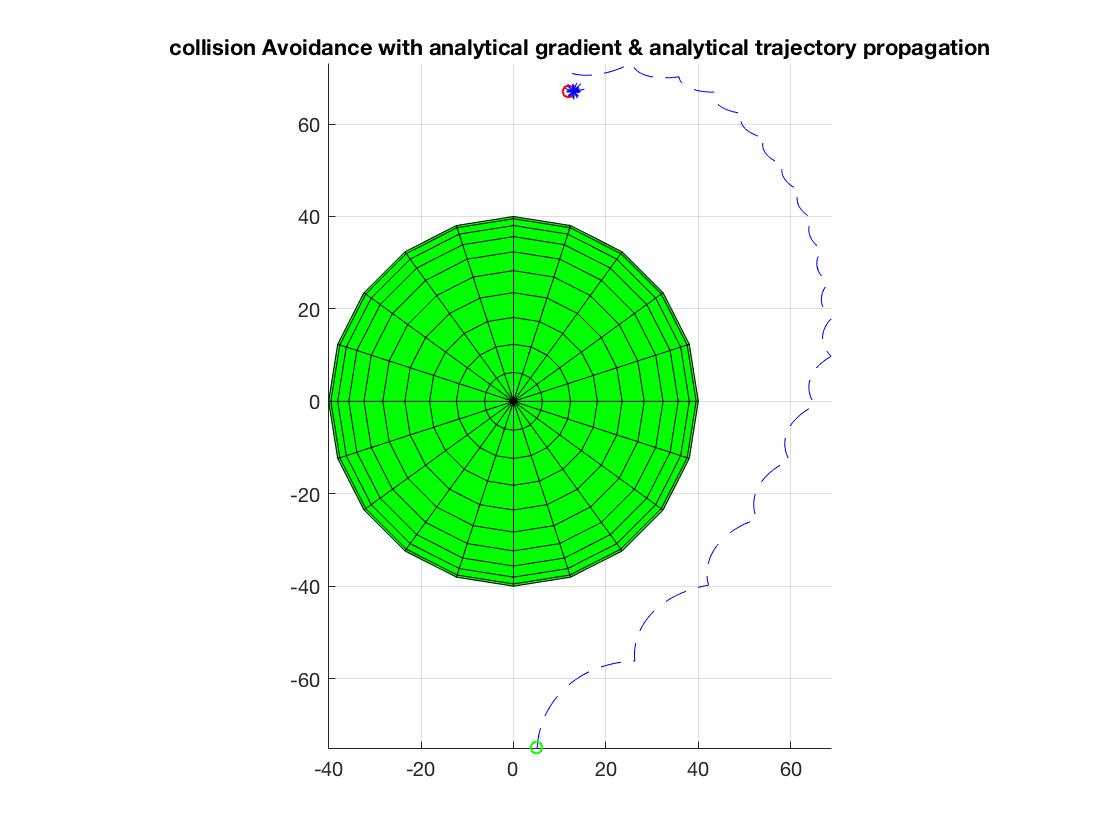
\includegraphics[width=10cm]{APF.jpg}
 		
 	\end{center}
 \end{figure}

\section{Fitness, Neural-Network, Dynamic: Individual.m (class) }

Attempts:
\begin{itemize}
\item{1: 8HL,tanh, regressor  $, fitness = \{goal +0.25, collision = -norm(v)/V, out\_of\_box= -norm(r-r\_goal)/L -0.25\}$}
\item{2: 16HL,tanh, regressor $, fitness = \{goal +0.25, collision = -norm(v)/V, default= -norm(r-r\_goal)/L\}$}
\end{itemize}

\begin{equation}
\Delta V = W_o (tanh(Whl * \{r/L, v/V \ \}+ b_{hl}) + b_{o}
\end{equation}
\textbf{\textsl{Action $\Delta V$ ! evaluated every 10s!}}\\
\textbf{\textsl{Simulation stops if $norm(r) > L $ or  $norm(r-r\_goal) < 5m$ }}\\
\textbf{\textsl{Thershold: $ \lvert \Delta V \lvert <= 0.0529$ }}

\section{result1: [8HL-Neuron][DISCONTINUOUS FITNESS SCORE FUNCTION]: \\ best\_individual\_until\_now.m }

 
 \begin{figure}[H]
 	\begin{center}
 		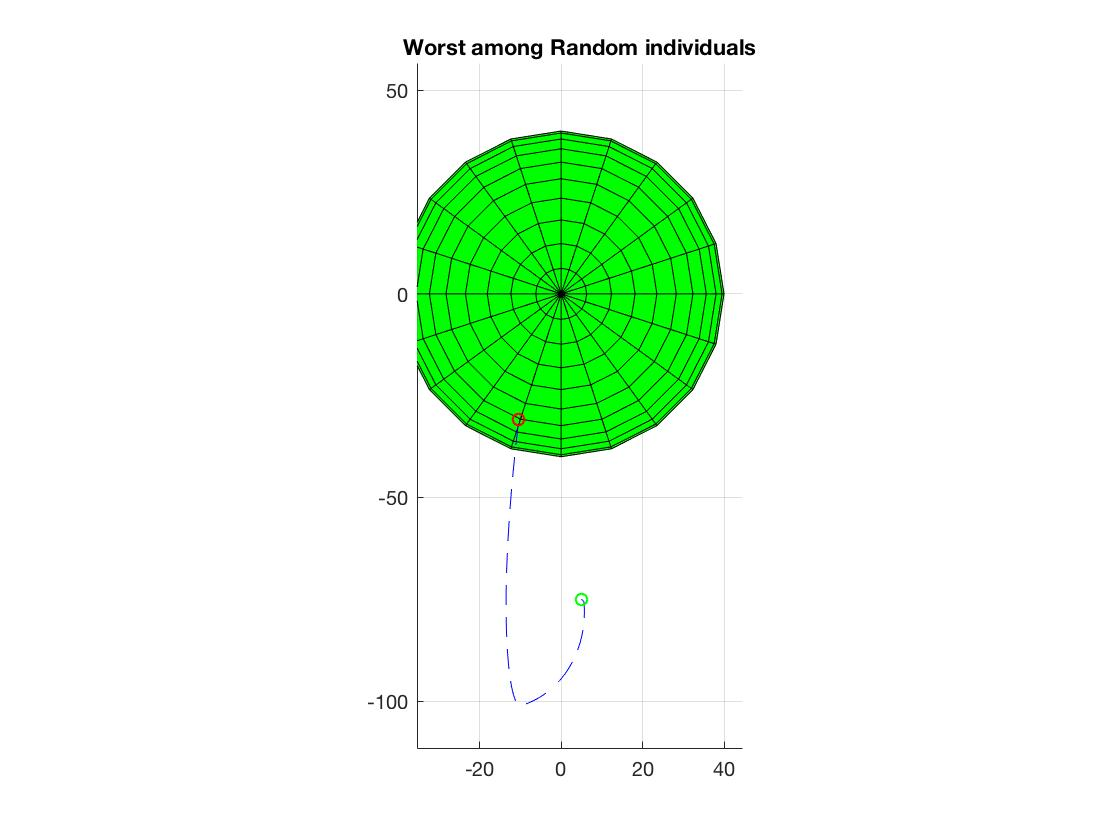
\includegraphics[width=10cm]{worst_among_random_Initial_individuals.jpg}
 		
 	\end{center}
 \end{figure}
 

\begin{figure}[H]
 	\begin{center}
 		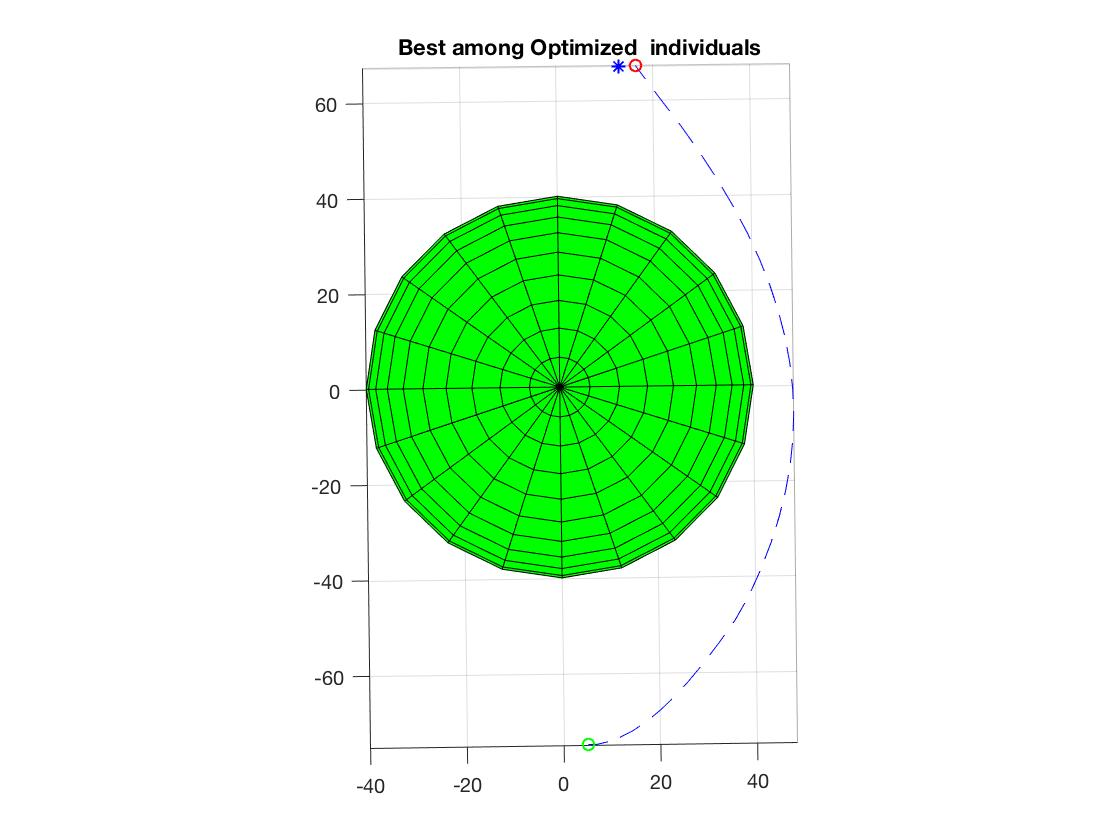
\includegraphics[width=10cm]{Best_result_ever.jpg}
 		
 	\end{center}
 \end{figure}
 
 
 \begin{figure}[H]
 	\begin{center}
 		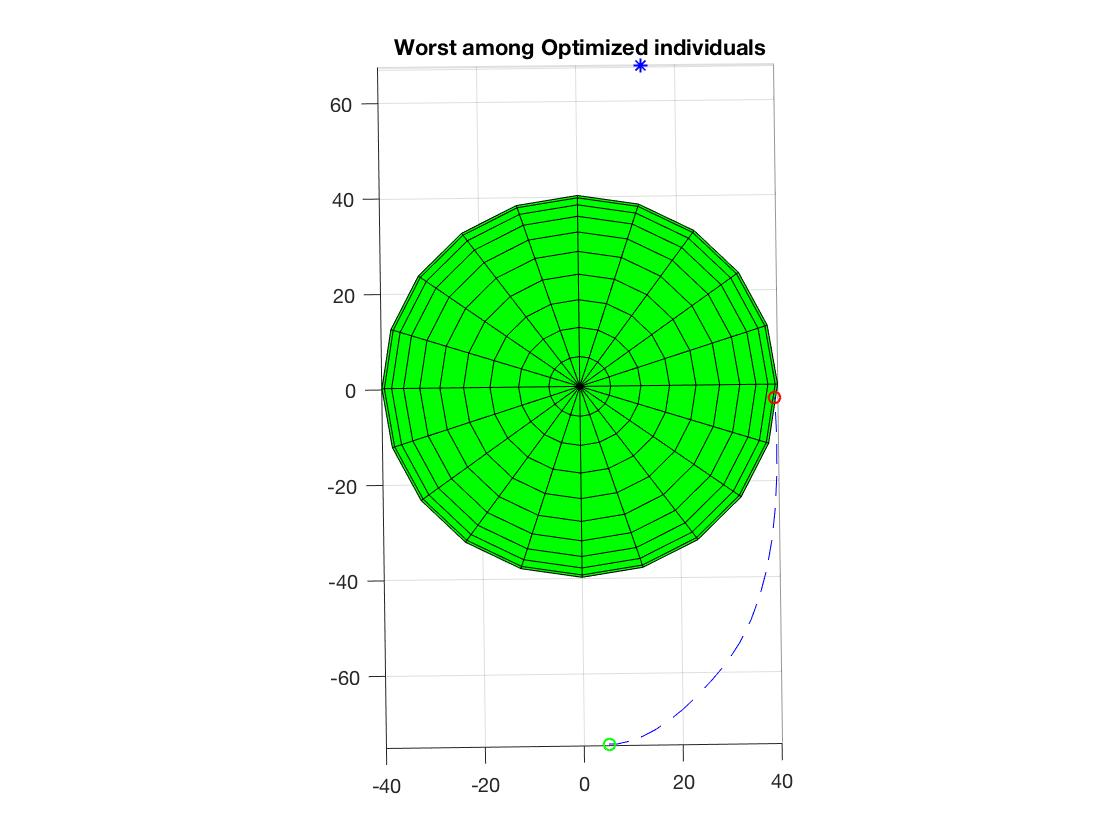
\includegraphics[width=10cm]{worst_among_optimized_individuals.jpg}
 		
 	\end{center}
 \end{figure}
 
 
 This trajectory appears to simulate a continuous thrust trajectory.

\section{Optimization considerations: createNextGeneration.m }


pseudo GA Optimization:\\

\textbf{ BREEDER:} $best\_sample $ Individuals among (sorted-by-score) evaluated population:
\textbf{CHILD-GENERATION: } Half neuron from (random-Breeder) DAD Hal neuron form (random-Breeder) MOM among breeder\\
\textbf{MUTATION: }  every weigth modified by the amount $rand([-0.001, +0.001])$ with a probability: $chance\_of\_mutation$\\
\textbf{GOLDEN-RULE:} 
\begin{equation}
(best\_sample + lucky\_few) / 2 * number\_of\_child = size\_population
\end{equation}
\\

\textbf{Algorithm:\\ }  
	$$populationSorted = computePerfPopulation(individuals);$$
    
	$$nextBreeders = selectFromPopulation(populationSorted,individuals,best\_samples, lucky\_few);$$
    
	$$nextPopulation = createChildren(nextBreeders, n\_children);$$
 
	$$nextGeneration = mutatePopulation(nextPopulation, chance\_of\_mutation);$$
	
	
\textbf{Program: \\}
generation = 10;
% SUPER-KEY-POINT: (best_sample + lucky_few) / 2 * number_of_child = size_population
$$while(generation > 1)$$
  
    $$populationNext = createNextGeneration(population, best\_samples, lucky\_few,number\_of\_child,chance\_of\_mutation);$$
  
    $$population = populationNext;$$
  
    $$generation = generation -1;$$
    
$$end  $$


Population size is kept the same along optimization =>?? Could be acceptable an elimination after a certain generation ??


 

\section{Next steps:}

\begin{itemize}
\item{implement output neurons as 'classifiers' $sigmoid$ or Biased output condition like \textsl{FIRE/NO-FIRE}}
\item{Train populations on modifying environments}
\item{Train from different initial conditions}
\item{train on a complex obstacle}
\end{itemize}









     \begin{thebibliography}{}
     

 


\bibitem{REINF_FINE}
\textit{Reinforcement Learning for Spacecraft Maneuvering Near Small Bodies}
Stefan Willis
, Dario Izzo
, Daniel Hennes
AAS/AIAA Space Flight Mechanics Meeting, Napa, CA in February 14-18, 2016
\bibitem{REINF1}
\textit{Self-supervised learning as an enabling technology
for future space exploration robots: ISS experiments}
Kevin van Hecke*a, Guido C.H.E. de Croon*a, Daniel HennesbTimothy P. Setterfieldc, Alvar Saenz-Oteroc, and Dario Izzo.
67-th International Astronautical Congress (IAC), Guadalajara, Mexico, 26-30 September 2016.

\bibitem{REINF_UAV}
\textit{Trajectory Optimization for Autonomous Flying
Base Station via Reinforcement Learning}
Harald Bayerlein, Paul de Kerret, and David Gesbert
Communication Systems Department, EURECOM
Sophia Antipolis, France

\bibitem{REINF_WAT}
\textit{Reinforcement Learning-based Motion Planning of a Triangular
Floating Platform under Environmental Disturbances}
Konstantinos Tziortziotis, Kostas Vlachos, Member, 24th Mediterranean Conference on Control and Automation (MED)
June 21-24, 2016, Athens, Greece

      \end{thebibliography}


\end{document}